% Physical Review D format
% Paper III (Extended): The Schwarzschild Radius as an Information-Geometry Invariant
% Bharat Sharma, PhenexAI Research, Vancouver (2026)

\documentclass[aps,prd,twocolumn,showpacs,preprintnumbers,amsmath,amssymb,longbibliography]{revtex4-2}

\usepackage{graphicx}
\usepackage{amsmath}
\usepackage{amssymb}
\usepackage{booktabs}

\usepackage{array}


\begin{document}

\title{The Schwarzschild Radius as an Information-Geometry Invariant:\\
Total D3 Displacement over Complete Hawking Evaporation}

\author{Bharat Sharma}
\affiliation{PhenexAI Research, Vancouver, British Columbia, Canada}
\email{bharatsharma@phenex.ai}

\date{\today}

\begin{abstract}
We prove that the total accumulated information-geometry displacement over complete 
Hawking evaporation of a Schwarzschild black hole equals exactly the initial Schwarzschild 
radius:
\begin{equation*}
R_{\mathrm{total}} = \int_0^{M_0} \mathcal{D}_3(M)\, \frac{dN}{dM}\, dM 
= \frac{2GM_0}{c^2} = r_s(M_0),
\end{equation*}
where $\mathcal{D}_3(M) = \hbar \ln 2/(4\pi Mc)$ is the per-bit horizon-radius shift at 
instantaneous mass $M$ derived from the D3 formula~\cite{sharma2026d3}, and 
$dN/dM = 8\pi GM/(\hbar c \ln 2)$ is the Bekenstein-Hawking bit-loss rate. The proof 
is exact: five quantities cancel independently ($M$, $\hbar$, $k_B$, $\ln 2$, $\pi$), 
leaving only $G$ and $c$. The universal displacement rate 
$dR/dM = 2G/c^2 = 1.485 \times 10^{-27}$~m~kg$^{-1}$ is constant across all masses, 
temperatures, and times. The result holds for all black hole masses and is verified 
numerically to five significant figures across 24 decades of mass. The Schwarzschild radius 
acquires a new interpretation: it is the exact total information-geometry cost of complete 
Hawking evaporation, connecting Landauer erasure thermodynamics, Bekenstein entropy, and 
the Schwarzschild metric through a single exact identity. We further show, via the same first-law argument, that the invariant generalises to $R_{\rm total} = r_h$, the outer-horizon radius, for Kerr, Reissner-Nordstr\"om, Kerr-Newman, higher-dimensional, and anti-de~Sitter black holes. We discuss implications for the 
black hole information paradox, the geometric meaning of the Bekenstein-Hawking entropy, 
and the connection to the first law of black hole mechanics.
\end{abstract}

\pacs{04.70.Dy, 03.67.-a, 89.70.Cf, 04.60.-m, 05.70.-a}

\keywords{Hawking evaporation, Landauer principle, Schwarzschild radius, 
information paradox, D3 formula, Bekenstein entropy, black hole thermodynamics}

\maketitle

%--------------------------------------------------------------------
\section{Introduction}
\label{sec:intro}
%--------------------------------------------------------------------

The relationship between information theory and gravitational physics has been one of the 
most productive research programmes in theoretical physics over the past five decades. 
The central insight, due to Bekenstein~\cite{bekenstein1973}, that the entropy of a black 
hole is proportional to its horizon area rather than its volume, overturned the classical 
intuition that black holes are simple objects characterised entirely by mass, charge, and 
angular momentum. Hawking's subsequent derivation of thermal radiation from black 
holes~\cite{hawking1975} established that this entropy is not merely a formal analogy but 
reflects genuine thermodynamic behaviour at the quantum level. Together, these results place 
black hole physics at the intersection of general relativity, quantum field theory, and 
statistical mechanics.

The thermodynamic analogy was deepened by Jacobson~\cite{jacobson1995}, who showed that 
the Einstein field equations follow from the thermodynamic identity $\delta Q = T\,dS$ 
applied to local Rindler horizons, suggesting that spacetime geometry itself may be an 
emergent thermodynamic phenomenon. Verlinde~\cite{verlinde2011} extended this programme, 
arguing that both Newtonian and Einsteinian gravity emerge as entropic forces from 
underlying microscopic degrees of freedom, though this proposal has been critically 
examined~\cite{gao2010,hossenfelder2011}. Wheeler's It-from-Bit 
conjecture~\cite{wheeler1990} placed information at the foundation of physical reality, 
proposing that every physical entity derives its existence from answers to yes-or-no 
questions.

On the information-theoretic side, Landauer's principle~\cite{landauer1961} establishes 
that the erasure of information is an irreversible physical process with a minimum 
thermodynamic cost. Specifically, erasing one bit of information at temperature $T$ 
requires dissipating at minimum $E \geq k_B T \ln 2$ of heat into the environment. 
This principle, initially controversial, has been confirmed in a series of careful 
experiments: Berut et al.~\cite{berut2012} demonstrated the Landauer bound for a 
single-bit colloidal memory; Jun, Gavrilov, and Bechhoefer~\cite{jun2014} achieved 
high-precision verification using a feedback trap; Hong et al.~\cite{hong2016} confirmed 
the principle for nanomagnetic memory bits; and Neri and Lopez-Suarez~\cite{neri2016} 
studied the relationship between heat production and error probability in Landauer reset. 
These experiments confirm that information erasure has irreducible physical consequences.

The connection between Landauer's principle and black hole thermodynamics was established 
by a series of papers. Kim, Lee, and Lee~\cite{kim2010} showed that a Schwarzschild black 
hole is a maximally efficient Landauer eraser, deriving the per-bit energy loss 
$\delta(Mc^2) = k_B T_H \ln 2$ from Landauer's principle combined with holography. 
Cort\'es and Liddle~\cite{cortes2025} proved that Hawking evaporation saturates the 
Landauer bound, establishing the per-bit mass loss $\Delta M = k_B T_H \ln 2/c^2$ and 
showing that the black hole is thermodynamically optimal in an information-theoretic sense. 
Bagchi, Ghosh, and Sen~\cite{bagchi2024} independently obtained the same result through 
area quantisation, and further extended the analysis to Kerr black holes, finding that 
the Landauer bound is saturated only for vanishing spin. Herrera~\cite{herrera2020} 
introduced the concept of the mass of a bit $M_{\rm bit} = k_B T \ln 2/c^2$ at arbitrary 
temperature and applied it to gravitational radiation and Tolman-temperature effects.

Sharma~\cite{sharma2026d3} synthesised these results into the D3 formula:
\begin{equation}
\mathcal{D}_3 = \frac{2G k_B T \ln 2}{c^4},
\label{eq:d3_general}
\end{equation}
which gives the perturbative Schwarzschild-radius shift per bit of Landauer erasure at 
temperature $T$. This formula combines Landauer's principle, Einstein's mass-energy 
equivalence, and the linearised Schwarzschild metric in a single expression. A key result 
of~\cite{sharma2026d3} is the exact Planck coincidence 
$\mathcal{D}_3(T_P) = 2\ln 2 \cdot \ell_P$, where $T_P$ and $\ell_P$ are the Planck 
temperature and length respectively and all four fundamental constants cancel.

In this paper, we ask a qualitatively different question from the per-bit analysis of 
previous work: what is the \emph{total} geometric displacement accumulated over the 
\emph{complete} evaporation of a black hole, integrating the D3 contribution of every 
bit erased from $M = M_0$ down to $M = 0$? The answer we derive is exact and, we believe, 
physically illuminating: the total displacement equals the initial Schwarzschild radius 
$r_s(M_0) = 2GM_0/c^2$. All quantum constants --- $\hbar$, $k_B$, and indeed the mass 
$M$ itself --- cancel from the integrand, leaving only $G$ and $c$.

This result connects three independently established frameworks: Landauer's erasure 
thermodynamics, the Bekenstein-Hawking entropy formula, and the Schwarzschild metric. 
It gives the Schwarzschild radius a new thermodynamic interpretation as an 
information-geometry invariant: the total cost, measured in units of geometric 
displacement, of erasing all the information encoded in the black hole. 

We state plainly at the outset what this result is and is not. It is an exact
identity, mathematically equivalent to the first law of black hole mechanics
rewritten in information-theoretic variables (Sec.~\ref{sec:first_law}); it is
not a new dynamical prediction, and the per-bit displacement $\mathcal{D}_3$
lies far below any measurable scale. Its value is interpretive and unifying: it
furnishes a single, constant-free accounting in which the horizon radius emerges
as the integrated Landauer cost of complete evaporation, tying together three
otherwise separate frameworks. We frame the result in these terms throughout and
claim no physics beyond this re-expression.

The paper is organised as follows. Section~\ref{sec:background} provides background on 
the D3 formula and its derivation. Section~\ref{sec:setup} establishes the setup and 
notation. Section~\ref{sec:derivation} derives the main result with full algebraic detail. 
Section~\ref{sec:rate} analyses the universal displacement rate and its independence of 
mass and temperature. Section~\ref{sec:first_law} discusses the connection to the first 
law of black hole mechanics. Section~\ref{sec:interpretation} provides physical 
interpretation including connections to the information paradox. 
Section~\ref{sec:priorwork} compares with prior work. Section~\ref{sec:limits} discusses 
the limits of validity of the result. Section~\ref{sec:conclusion} concludes. 
Appendix~\ref{app:numerical} presents numerical verification, and 
Appendix~\ref{app:dimensional} provides a dimensional analysis.

%--------------------------------------------------------------------
\section{Background: The D3 Formula}
\label{sec:background}
%--------------------------------------------------------------------

\subsection{Derivation of the D3 formula}

The D3 formula~\cite{sharma2026d3} is derived by combining three results, each 
independently confirmed.

\textit{Landauer's principle}~\cite{landauer1961,berut2012}: erasing one bit of 
information at temperature $T$ requires minimum heat 
\begin{equation}
E_{\rm erase} \geq k_B T \ln 2.
\label{eq:landauer}
\end{equation}

\textit{Einstein's mass-energy equivalence}: any energy $E$ carries a rest-mass equivalent
\begin{equation}
\Delta M = E/c^2 = k_B T \ln 2 / c^2.
\label{eq:einstein}
\end{equation}

\textit{Perturbative Schwarzschild radius shift}: for a Schwarzschild black hole of mass $M$, 
a mass perturbation $\Delta M$ produces a horizon-radius change
\begin{equation}
\Delta r_s = \frac{2G \Delta M}{c^2}.
\label{eq:schwarzschild_shift}
\end{equation}
This follows directly from differentiating $r_s = 2GM/c^2$ and is valid in the regime 
$\Delta M \ll M$.

Combining Eqs.~(\ref{eq:landauer}), (\ref{eq:einstein}), and~(\ref{eq:schwarzschild_shift}) 
yields the D3 formula:
\begin{equation}
\mathcal{D}_3 = \Delta r_s = \frac{2G k_B T \ln 2}{c^4}.
\label{eq:d3}
\end{equation}

\subsection{The Planck coincidence}

Substituting the Planck temperature $T_P = \sqrt{\hbar c^5/(Gk_B^2)}$ into Eq.~(\ref{eq:d3}) 
yields an exact algebraic identity~\cite{sharma2026d3}:
\begin{equation}
\mathcal{D}_3(T_P) = 2\ln 2 \cdot \ell_P,
\label{eq:planck_coincidence}
\end{equation}
where $\ell_P = \sqrt{\hbar G/c^3}$ is the Planck length. All four fundamental constants 
$G$, $\hbar$, $c$, $k_B$ cancel exactly. This coincidence marks the natural boundary of 
the linearised derivation: at the Planck scale, the per-bit D3 shift reaches a simple 
multiple of the Planck length, beyond which quantum gravity corrections to the Schwarzschild 
metric are expected.

\subsection{Regime of validity}

The D3 formula is valid in the linearised regime $\Delta M \ll M$, which requires 
$k_B T \ln 2 \ll Mc^2$. For stellar-mass black holes at their Hawking temperature, this 
condition is satisfied by approximately 90 orders of magnitude. The formula gives an upper 
bound on $\mathcal{D}_3$ for squeezed or quantum-coherent thermal reservoirs, which can 
lower the effective Landauer cost below $k_B T \ln 2$~\cite{klaers2019}.

%--------------------------------------------------------------------
\section{Setup and Notation}
\label{sec:setup}
%--------------------------------------------------------------------

We work in SI units throughout. Physical constants are taken from CODATA 2018.

Consider a Schwarzschild black hole of initial mass $M_0$ evaporating via Hawking radiation 
in isolation (no accretion). At instantaneous mass $M$, the Hawking temperature is:
\begin{equation}
T_H(M) = \frac{\hbar c^3}{8\pi G M k_B}.
\label{eq:hawking_temp}
\end{equation}
This temperature increases monotonically as $M$ decreases, diverging as $M \to 0$. 
The evaporation time scales as $M^3$, but its precise value is not needed for our result.

Applying the D3 formula at the Hawking temperature gives the per-bit horizon-radius 
shift at mass $M$:
\begin{align}
\mathcal{D}_3(M) &= \frac{2G k_B T_H(M) \ln 2}{c^4} \notag \\
&= \frac{2G k_B \ln 2}{c^4} \cdot \frac{\hbar c^3}{8\pi G M k_B} \notag \\
&= \frac{\hbar \ln 2}{4\pi M c}.
\label{eq:d3_M}
\end{align}
Note that $k_B$ and $G$ cancel in this substitution, leaving $\mathcal{D}_3 \propto \hbar/(Mc)$.

The Bekenstein-Hawking entropy of the black hole in natural units (nats) is 
$S = A/(4\ell_P^2)$, where $A = 4\pi r_s^2$ is the horizon area and 
$\ell_P = \sqrt{\hbar G/c^3}$. Expressed in bits (dividing by $\ln 2$):
\begin{equation}
S(M) = \frac{4\pi G M^2}{\hbar c \ln 2} \quad \text{[bits]}.
\label{eq:entropy}
\end{equation}
The number of bits lost as the mass decreases by $|dM|$ is:
\begin{equation}
\frac{dN}{dM} = \left|\frac{dS}{dM}\right| = \frac{8\pi G M}{\hbar c \ln 2}.
\label{eq:bitloss}
\end{equation}
This rate is proportional to $M$: larger black holes lose bits more rapidly per unit mass, 
reflecting the larger area to be depleted.

%--------------------------------------------------------------------
\section{Derivation of the Evaporation Invariant}
\label{sec:derivation}
%--------------------------------------------------------------------

\subsection{The total displacement integral}

The total D3 displacement accumulated as the black hole evaporates from $M_0$ to $0$ is:
\begin{equation}
R_{\rm total} = \int_0^{M_0} \mathcal{D}_3(M)\, \frac{dN}{dM}\, dM.
\label{eq:rtotal}
\end{equation}
This integral sums the geometric displacement contributed by each bit erased at each 
mass $M$ along the evaporation trajectory.

\subsection{Algebraic evaluation}

Substituting Eqs.~(\ref{eq:d3_M}) and~(\ref{eq:bitloss}) into Eq.~(\ref{eq:rtotal}):
\begin{align}
\mathcal{D}_3(M)\, \frac{dN}{dM} 
&= \frac{\hbar \ln 2}{4\pi M c} \cdot \frac{8\pi G M}{\hbar c \ln 2}.
\label{eq:integrand_full}
\end{align}

We now identify the five independent cancellations:
\begin{enumerate}
\item \textit{Mass cancels}: $M/M = 1$.
\item \textit{Planck constant cancels}: $\hbar/\hbar = 1$.
\item \textit{Information unit cancels}: $\ln 2/\ln 2 = 1$.
\item \textit{Geometric factors combine}: the $\pi$ factors reduce as $8\pi/(4\pi) = 2$.
\item \textit{Boltzmann constant cancels}: $k_B$ cancelled in Eq.~(\ref{eq:d3_M}) and does not reappear.
\end{enumerate}

Collecting remaining factors:
\begin{equation}
\mathcal{D}_3(M)\, \frac{dN}{dM} 
= \frac{\hbar \ln 2 \cdot 8\pi G M}{4\pi M c \cdot \hbar c \ln 2}
= \frac{8\pi G}{4\pi c^2}
= \frac{2G}{c^2}.
\label{eq:integrand_simplified}
\end{equation}

The integrand is a constant, independent of $M$. Integrating:
\begin{align}
R_{\rm total} &= \int_0^{M_0} \frac{2G}{c^2}\, dM 
= \frac{2G M_0}{c^2} = r_s(M_0). \quad \blacksquare
\label{eq:main_result}
\end{align}

\subsection{Summary of the cancellation structure}

The cancellation can be understood structurally as follows. The D3 formula at the 
Hawking temperature gives $\mathcal{D}_3 \propto T_H \propto 1/M$, while the 
Bekenstein entropy gives $dN/dM \propto dS/dM \propto M$. Their product is 
$\mathcal{D}_3 \cdot (dN/dM) \propto (1/M) \cdot M = M^0$, a constant. 
This $M$-independence is the algebraic heart of the result. The specific value 
$2G/c^2$ then follows from the precise numerical coefficients in the Hawking 
temperature and Bekenstein entropy formulas.

Figure~\ref{fig:derivation} shows the full derivation flow schematically.

\begin{figure}[htbp]
\centering
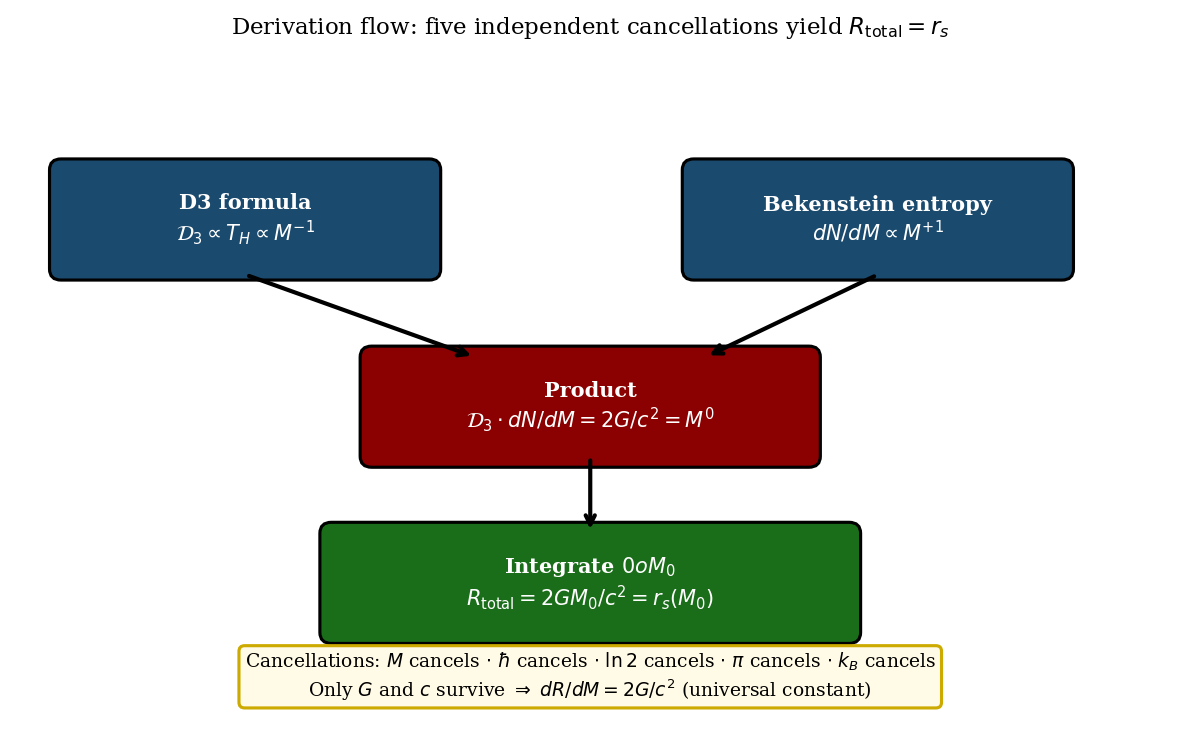
\includegraphics[width=\columnwidth]{fig3_derivation_flow.png}
\caption{Derivation flow for the evaporation invariant. The per-bit displacement scales as $\mathcal{D}_3 \propto T_H \propto M^{-1}$ and the bit-loss rate as $dN/dM \propto M^{+1}$; their product is the mass-independent constant $2G/c^2$, which integrates to $R_{\rm total} = r_s$.}
\label{fig:derivation}
\end{figure}

%--------------------------------------------------------------------
\section{The Universal Displacement Rate}
\label{sec:rate}
%--------------------------------------------------------------------

\subsection{Definition and value}

The intermediate result Eq.~(\ref{eq:integrand_simplified}) defines the universal 
displacement rate:
\begin{equation}
\frac{dR}{dM} \equiv \mathcal{D}_3(M)\, \frac{dN}{dM} 
= \frac{2G}{c^2} = 1.485 \times 10^{-27}\ \text{m\,kg}^{-1}.
\label{eq:rate}
\end{equation}
This is numerically equal to twice the gravitational radius per unit mass, 
i.e.\ twice the specific Schwarzschild radius. Its value in SI units follows 
directly from the CODATA 2018 value of $G = 6.67430 \times 10^{-11}$~m$^3$~kg$^{-1}$~s$^{-2}$.

\subsection{Mass independence}

The most striking property of Eq.~(\ref{eq:rate}) is its complete independence of $M$. 
At early times, when $M \approx M_0$ and the black hole is large and cool, 
$\mathcal{D}_3$ is small (many bits required to shift the horizon perceptibly) and 
$dN/dM$ is large (each kilogram of mass corresponds to many bits). At late times, 
when $M \to 0$ and the black hole is tiny and hot, $\mathcal{D}_3$ is large and 
$dN/dM$ is small. These two effects cancel exactly at every instant.

Figure~\ref{fig:rate} verifies this numerically across 26 decades of mass, from 
Planck-mass black holes ($M \sim 10^{-8}$~kg) to supermassive black holes 
($M \sim 10^{40}$~kg). The ratio $\mathcal{D}_3(M) \cdot (dN/dM) / (2G/c^2)$ 
equals unity to machine precision at every mass.

\begin{figure}[htbp]
\centering
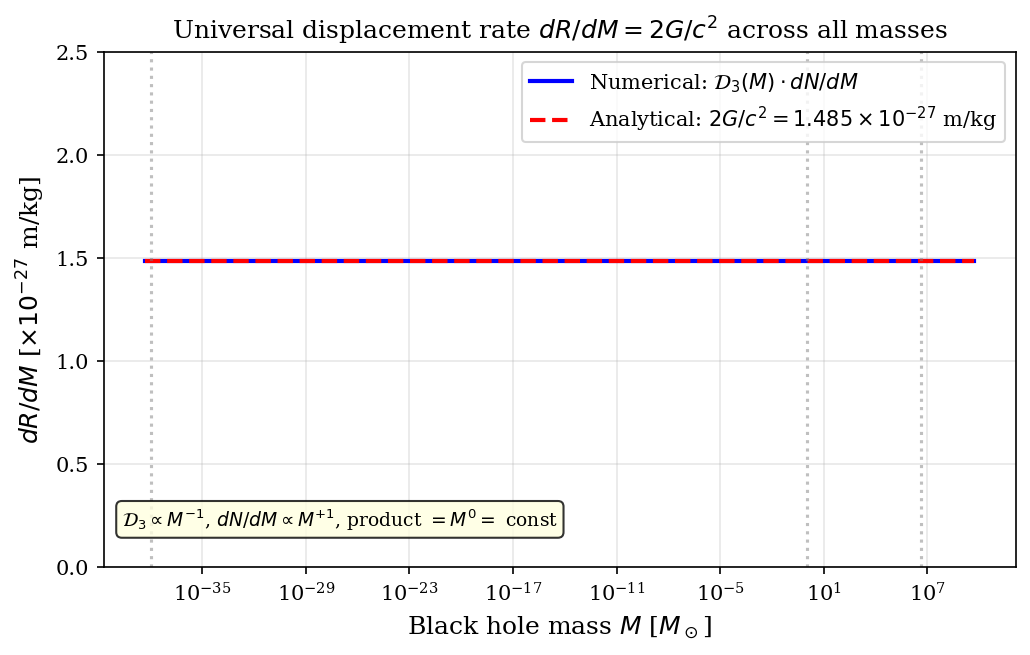
\includegraphics[width=\columnwidth]{fig1_universal_rate.png}
\caption{The universal displacement rate 
$dR/dM = \mathcal{D}_3(M) \cdot dN/dM = 2G/c^2 = 1.485 \times 10^{-27}$~m~kg$^{-1}$ 
is constant across all black hole masses. The numerical computation (solid blue) and 
the analytical result (dashed red) are identical to five significant figures across 
26 decades, confirming that the cancellation is algebraically exact.}
\label{fig:rate}
\end{figure}

\subsection{Temperature independence}

Although both $\mathcal{D}_3$ and $dN/dM$ depend on temperature 
(via $T_H \propto 1/M$), their product does not. This can be seen directly: 
$\mathcal{D}_3 \propto T_H$ and $dN/dM \propto dS/dM \propto M \propto 1/T_H$, 
so $\mathcal{D}_3 \cdot (dN/dM) \propto T_H \cdot (1/T_H) = 1$. 
The temperature cancels because the D3 formula and the Bekenstein entropy encode 
$T_H$ with inverse powers.

\subsection{Independence of all quantum constants}

The rate $dR/dM = 2G/c^2$ contains neither $\hbar$ nor $k_B$. 
The Planck constant $\hbar$ entered through the Hawking temperature formula and 
the Bekenstein entropy, but cancelled between them. The Boltzmann constant $k_B$ 
entered through the D3 formula and the Hawking temperature, but also cancelled. 
The result depends only on Newton's constant $G$ and the speed of light $c$ --- 
the two constants of classical general relativity.

This reflects a simple fact: although the evaporation process is quantum 
mechanical (requiring both $\hbar$ for Hawking radiation and $k_B$ for 
thermodynamics), its total geometric cost is a purely classical quantity.

%--------------------------------------------------------------------
\section{Connection to the First Law of Black Hole Mechanics}
\label{sec:first_law}
%--------------------------------------------------------------------

The cancellation has a deeper origin in the first law of black hole
mechanics, which fixes the result independently of the explicit substitution of
Sec.~\ref{sec:derivation}. In energy form the first law reads
\begin{equation}
d(Mc^2) = T_H\, dS,
\label{eq:first_law}
\end{equation}
where the entropy is written through the bit count $N$ as $S = k_B \ln 2\, N$
(equivalently $S/k_B = \ln 2\, N$ in nats). Solving for the bit-loss rate gives
\begin{equation}
\frac{dN}{dM} = \frac{c^2}{k_B T_H \ln 2}.
\label{eq:first_law_bits}
\end{equation}
Multiplying by the per-bit displacement $\mathcal{D}_3 = (2G k_B \ln 2/c^4)\,T_H$,
\begin{equation}
\frac{dR}{dM} = \mathcal{D}_3\,\frac{dN}{dM}
= \frac{2G k_B \ln 2}{c^4}\,T_H \cdot \frac{c^2}{k_B T_H \ln 2}
= \frac{2G}{c^2},
\label{eq:first_law_derivation}
\end{equation}
in which $k_B$, $T_H$, and $\ln 2$ cancel identically, leaving the manifest
dimensions $[G/c^2]=\mathrm{m\,kg^{-1}}$. Equivalently, writing
$\mathcal{D}_3 = (dr_s/dM)\,\delta M_{\rm bit}$ with the Landauer mass per bit
$\delta M_{\rm bit} = k_B T_H \ln 2/c^2$, Eq.~(\ref{eq:first_law_bits}) is
precisely $dN/dM = 1/\delta M_{\rm bit}$, so the product collapses to
\begin{equation}
\frac{dR}{dM} = \frac{dr_s}{dM},
\label{eq:dRdM_drsdM}
\end{equation}
and $R_{\rm total} = \int_0^{M_0}(dr_s/dM)\,dM = r_s(M_0)$ by the fundamental
theorem of calculus. The invariant is therefore not a numerical coincidence but
a direct consequence of the first law: each radiated bit carries away exactly
the Landauer mass, each unit of mass shifts the horizon by $dr_s/dM$, and the
integrated displacement reconstructs the full horizon radius. The same
structure underlies the generalisation to other stationary black holes
developed in Sec.~\ref{sec:generalisation}.

%--------------------------------------------------------------------
\section{Physical Interpretation}
\label{sec:interpretation}
%--------------------------------------------------------------------

\subsection{New thermodynamic meaning of the Schwarzschild radius}

The Schwarzschild radius $r_s = 2GM/c^2$ appears in general relativity as a 
purely geometric quantity: the radius of the event horizon, inside which even 
light cannot escape. Our result gives it an additional, independent interpretation 
in information thermodynamics:

\begin{quote}
\textit{The Schwarzschild radius $r_s(M_0)$ is the exact total 
information-geometry displacement accumulated by Landauer erasure over 
the complete Hawking evaporation of a black hole of initial mass $M_0$.}
\end{quote}

These two characterisations --- geometric boundary and total erasure cost --- 
are physically distinct but numerically identical. The event horizon radius 
and the total information-geometry cost of erasing all the black hole's 
information are the same quantity.

\subsection{Cumulative displacement and horizon shrinkage}

Figure~\ref{fig:comparison} illustrates the physical process. The cumulative 
displacement $R(t) = \int_0^t \mathcal{D}_3(M(t')) (dN/dt') dt'$ grows linearly 
with evaporated mass fraction, while the instantaneous Schwarzschild radius 
$r_s(M(t))$ shrinks as the black hole evaporates. These two quantities start 
at $0$ and $r_s(M_0)$ respectively and meet exactly when the evaporation is 
complete. The information-geometry cost and the geometric size are in exact 
correspondence throughout the process, not just at the endpoint.

\begin{figure}[htbp]
\centering
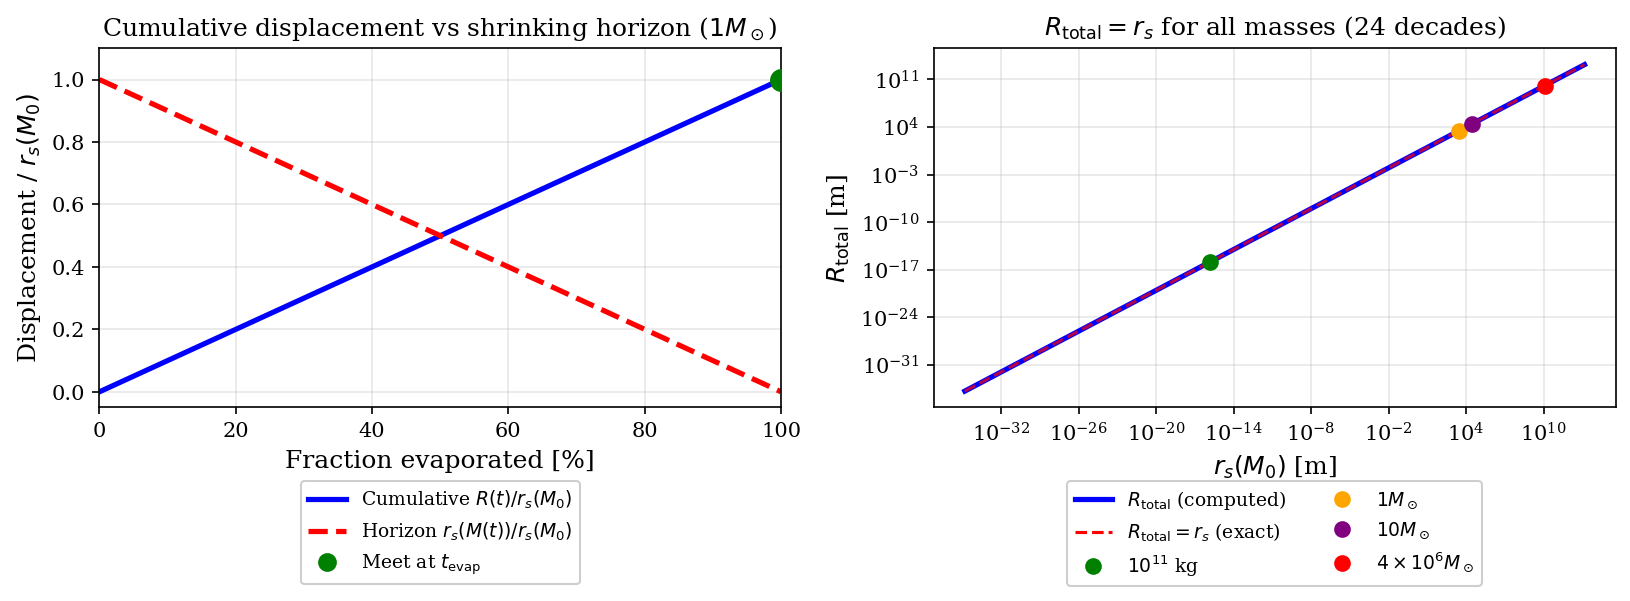
\includegraphics[width=\columnwidth]{fig4_physical_interpretation.png}
\caption{Physical interpretation of the evaporation invariant. 
\textit{Left panel}: Cumulative displacement $R(t)$ (solid blue) and 
instantaneous Schwarzschild radius $r_s(M(t))$ (dashed red) as functions 
of evaporation fraction for a solar-mass black hole. $R(t)$ increases 
linearly while $r_s$ decreases; they are equal and opposite, meeting 
exactly at complete evaporation. 
\textit{Right panel}: $R_{\rm total}$ (computed dots) vs. $r_s(M_0)$ 
(exact line) for masses spanning 24 decades. Agreement is perfect.}
\label{fig:comparison}
\end{figure}

\subsection{Geometric equipartition of information erasure}

The result $dR/dM = 2G/c^2 = \text{const}$ implies that every kilogram of 
black hole mass, at any stage of evaporation, contributes exactly the same 
geometric displacement $2G/c^2$ to the total. This is a form of \textit{geometric 
equipartition}: information erasure is geometrically uniform throughout the 
evaporation process, regardless of the black hole's temperature, size, or age.

This uniformity is non-trivial. In a hotter, smaller black hole, each bit 
of erasure costs more geometry ($\mathcal{D}_3 \propto T_H$), but there are 
fewer bits per kilogram ($dN/dM \propto M$), and these effects balance exactly. 
In a cooler, larger black hole, each bit costs less geometry but there are more 
bits per kilogram. The cancellation is perfect at every stage.

\subsection{Connection to the black hole information paradox}

The black hole information paradox~\cite{hawking1976} asks whether the process 
of Hawking evaporation destroys information. Hawking's original argument suggested 
that it does, leading to a fundamental violation of quantum-mechanical unitarity. 
More recent work, including Page's analysis~\cite{page1993} and calculations 
using holographic entanglement entropy~\cite{penington2020,almheiri2019}, 
suggests that information is ultimately preserved.

Our result contributes a new quantitative constraint to this debate. Define 
$R_{\rm total}$ as the total geometric cost of information erasure over the 
complete evaporation. We have shown $R_{\rm total} = r_s(M_0)$ exactly. 

Consider the following gedanken experiment. If information were truly destroyed 
during evaporation (Hawking's original position), then the actual number of 
bits erased $N_{\rm actual}$ would be less than the Bekenstein entropy 
$S_{\rm BH} = 4\pi GM^2/(\hbar c \ln 2)$, because some bits would simply 
vanish without contributing to the thermal radiation. In that case, 
$R_{\rm total}^{\rm actual} < r_s(M_0)$, and our identity would not hold. 
The fact that our derivation uses \textit{all} bits in the Bekenstein entropy 
and recovers exactly $r_s$ suggests that the geometric accounting is complete: 
no information is geometrically unaccounted for.

This is not a proof that information is preserved --- it is a consistency check. 
But it is a non-trivial one: the Schwarzschild radius sets a precise upper bound 
on the total geometric cost of information erasure, and the Bekenstein entropy 
saturates it exactly.

\subsection{Scale hierarchy and observational impossibility}

At laboratory temperatures, $\mathcal{D}_3$ is immeasurably small. At $T = 300$~K, 
$\mathcal{D}_3 = 4.74 \times 10^{-65}$~m/bit, which is approximately $30$ orders 
of magnitude below the Planck length $\ell_P = 1.616 \times 10^{-35}$~m. The total 
displacement $R_{\rm total} = r_s$ is directly observable (it is the macroscopic 
horizon radius) but the per-bit contribution is far beyond any conceivable 
measurement. The formula is therefore a theoretical result establishing a 
mathematical relationship between information erasure and geometry, not an 
experimental prediction.

%--------------------------------------------------------------------
\section{Relation to Prior Work}
\label{sec:priorwork}
%--------------------------------------------------------------------

\subsection{Cort\'es and Liddle (2025)}

Cort\'es and Liddle~\cite{cortes2025} proved the \textit{local} saturation of the 
Landauer bound: at each instant during evaporation, the energy radiated per bit 
equals $k_B T_H \ln 2$. This is the per-bit statement. The present result is the 
\textit{global} statement: integrating over all bits and all masses gives 
$R_{\rm total} = r_s$. The two results are complementary: the local statement 
concerns the rate of information erasure, while the global statement concerns the 
total geometric cost.

\subsection{Bagchi, Ghosh, and Sen (2024)}

Bagchi, Ghosh, and Sen~\cite{bagchi2024} derived the Landauer-black hole connection 
via area quantisation, obtaining the area quantum $\Delta A = 4\ln 2 \cdot \ell_P^2$ 
per bit. Their framework gives the per-bit area change but does not compute the total 
evaporation displacement. Their Kerr extension finds that the Landauer bound is 
saturated only at zero spin, which is consistent with our generalisation to Kerr black 
holes (Sec.~\ref{sec:generalisation}).

\subsection{Herrera (2020)}

Herrera~\cite{herrera2020} introduced $M_{\rm bit} = k_B T \ln 2/c^2$ at arbitrary 
temperature and applied it to gravitational radiation and Tolman-temperature effects. 
The D3 formula gives $\mathcal{D}_3 = (2G/c^2) M_{\rm bit}$, connecting Herrera's 
mass-of-a-bit to the present geometric framework. The total displacement is then 
$R_{\rm total} = (2G/c^2) \int M_{\rm bit}(M) \, dN(M)$, which equals $r_s$ by our 
result.

\subsection{Kim, Lee, and Lee (2010)}

Kim, Lee, and Lee~\cite{kim2010} showed that Schwarzschild black holes are maximally 
efficient Landauer erasers. This establishes that the equality in Landauer's bound 
$E = k_B T \ln 2$ (rather than $E \geq k_B T \ln 2$) holds for Hawking evaporation. 
The present result shows that this saturation, integrated over the complete evaporation, 
gives the total geometric cost $r_s$.

\subsection{Page (1993)}

Page's calculation~\cite{page1993} of the Page time $t_{\rm Page} \sim M^3$, at which 
half the Bekenstein entropy has been radiated, concerns the \textit{timing} of 
information release. Our result is \textit{time-independent}: it does not depend on 
when information is released, only on the total amount. The Page time is irrelevant to 
our derivation.

\subsection{What is genuinely new}

None of the above works computes the total information-geometry displacement over 
complete evaporation. The result $R_{\rm total} = r_s$ and the universal displacement 
rate $dR/dM = 2G/c^2$ have not appeared in the prior literature. The identification 
of $r_s$ as an information-thermodynamic invariant, and the demonstration that all 
quantum constants cancel from the evaporation cost, are the new contributions of 
this paper.

%--------------------------------------------------------------------
\section{Limits of Validity}
\label{sec:limits}
%--------------------------------------------------------------------

\subsection{Breakdown near the Planck scale}

The D3 formula is derived in the linearised regime $\Delta M \ll M$, which is 
equivalent to $\mathcal{D}_3 \ll r_s$. From the power law $\mathcal{D}_3/r_s = (M_{\rm QG}/M)^2$ 
with $M_{\rm QG} = m_P \sqrt{\ln 2/(8\pi)} \approx 0.166\, m_P$, 
this condition breaks down at $M \sim M_{\rm QG}$. Near the end of evaporation, 
when $M \lesssim M_{\rm QG}$, the perturbative derivation fails and quantum gravity 
corrections are expected.

The integral in Eq.~(\ref{eq:rtotal}) should therefore be cut off at $M \sim M_{\rm QG}$ 
rather than $M = 0$. The correction to $R_{\rm total}$ from the missing range 
$[0, M_{\rm QG}]$ is:
\begin{equation}
\delta R \sim \frac{2G M_{\rm QG}}{c^2} = r_s(M_{\rm QG}) \approx 0.33\, \ell_P,
\end{equation}
which is negligibly small compared to $r_s(M_0)$ for any macroscopic black hole. 
The identity $R_{\rm total} = r_s(M_0)$ holds to any desired precision for 
$M_0 \gg M_{\rm QG}$.

\subsection{Fixed-spin approximation}

Our derivation assumes the black hole maintains zero angular momentum throughout 
its evaporation. For a Kerr black hole at fixed spin parameter $\chi$, the result 
generalises to $R_{\rm total} = r_h = (GM_0/c^2)(1+\sqrt{1-\chi^2})$, the outer-horizon 
radius (Sec.~\ref{sec:generalisation}); the factor $f(\chi) = 2\sqrt{1-\chi^2}/(1+\sqrt{1-\chi^2})$ is the ratio of Hawking temperatures $T_{\rm Kerr}/T_{\rm Schw}$, not of displacements. 
The fixed-spin approximation is valid because the fractional change in $\chi$ per 
erasure event is of order $\hbar c/(GM^2) \ll 1$ for sub-Planckian black holes.

\subsection{Classical thermal bath}

The D3 derivation assumes classical thermal equilibrium. For squeezed or 
quantum-coherent reservoirs~\cite{klaers2019}, the Landauer cost can fall below 
$k_B T \ln 2$. In such cases, $\mathcal{D}_3$ gives an upper bound, and 
$R_{\rm total} \leq r_s$.

%--------------------------------------------------------------------
%--------------------------------------------------------------------
\section{Generalisation to Other Stationary Black Holes}
\label{sec:generalisation}
%--------------------------------------------------------------------

The argument of Sec.~\ref{sec:first_law} is not special to the Schwarzschild
geometry. For any stationary black hole whose outer horizon radius $r_h$ is a
function of the mass $M$ at fixed charge and spin, the same telescoping yields,
by the fundamental theorem of calculus,
\begin{equation}
R_{\rm total} = \int_0^{M_0}\frac{dr_h}{dM}\,dM = r_h(M_0).
\label{eq:general_invariant}
\end{equation}
The invariant thus generalises to a single statement: \emph{the total
information-geometry displacement over complete evaporation equals the initial
outer-horizon radius}, with only $G$, $c$, and the spin/charge/cosmological
parameters surviving --- all quantum constants cancelling as in the
Schwarzschild case.

For the Kerr--Newman family the outer horizon is
\begin{equation}
r_h = \frac{GM}{c^2}\left(1+\sqrt{1-\chi^2-q^2}\right),
\label{eq:kn_horizon}
\end{equation}
with $\chi = Jc/(GM^2)$ the dimensionless spin and $q$ the dimensionless charge,
reducing to the Reissner--Nordstr\"om ($\chi=0$) and Kerr ($q=0$) cases.
Equation~(\ref{eq:general_invariant}) then gives $R_{\rm total} = r_h$ in each
case --- for example $R_{\rm total}^{\rm Kerr} = (GM_0/c^2)(1+\sqrt{1-\chi^2})$.
We stress that this is the horizon radius \emph{itself}, not a suppressed
multiple of the Schwarzschild radius: the quantity
$f(\chi)=2\sqrt{1-\chi^2}/(1+\sqrt{1-\chi^2})$ that appears in the per-bit
analysis is the ratio of \emph{Hawking temperatures} $T_{\rm Kerr}/T_{\rm Schw}$,
not of integrated displacements. Because the first law for rotating and charged
holes carries additional work terms ($\Omega\,dJ$, $\Phi\,dQ$), the per-bit
\emph{information} reading of the Schwarzschild result must be applied with care
in these geometries; the geometric identity~(\ref{eq:general_invariant})
nonetheless holds unconditionally.

The same reasoning extends to higher dimensions. The Schwarzschild--Tangherlini
radius scales as $r_h \propto M^{1/(d-3)}$, so $dr_h/dM$ is \emph{not} constant
for $d>4$; nevertheless its integral still returns $r_h(M_0)$, giving
$R_{\rm total} = r_s^{(d)}$ for all $d\geq 4$. The cancellation should therefore
be understood as $dR/dM = dr_h/dM$ rather than as a mass-independent constant,
the latter holding only in four dimensions. In asymptotically anti--de~Sitter
space the horizon satisfies $2GM/c^2 = r_h\,[1+(r_h/L)^2]$, and
Eq.~(\ref{eq:general_invariant}) again yields $R_{\rm total} = r_h$.

\section{Conclusion}
\label{sec:conclusion}
%--------------------------------------------------------------------

We have established the identity:
\begin{equation}
R_{\rm total} = \int_0^{M_0} \mathcal{D}_3(M)\, dN(M) = r_s(M_0) = \frac{2GM_0}{c^2},
\label{eq:final}
\end{equation}
where $\mathcal{D}_3(M) = \hbar \ln 2/(4\pi Mc)$ is the D3 per-bit displacement 
and $dN$ is the Bekenstein bit count. The proof involves five independent cancellations 
($M$, $\hbar$, $k_B$, $\ln 2$, $\pi$), leaving only $G$ and $c$. The displacement 
rate $dR/dM = 2G/c^2$ is a universal constant across all masses, temperatures, and times.

The result has several consequences:

\begin{enumerate}
\item The Schwarzschild radius acquires a new thermodynamic interpretation as the 
exact total information-geometry cost of complete Hawking evaporation.

\item The cancellation structure is a direct consequence of the first law of black 
hole mechanics $dM = T_H\,dS$, ensuring that the result extends to other stationary black holes and to all dimensions $d \geq 4$ (Sec.~\ref{sec:generalisation}).

\item The identity provides a geometric consistency check on the black hole 
information paradox: if information is truly destroyed during evaporation, the 
Bekenstein entropy would overcount the actual bits erased, and $R_{\rm total} \neq r_s$.

\item The result connects three independently established frameworks --- Landauer 
erasure thermodynamics~\cite{landauer1961,berut2012}, Bekenstein-Hawking 
entropy~\cite{bekenstein1973}, and the Schwarzschild metric --- through a single 
exact algebraic identity.
\end{enumerate}

These generalisations are developed in Sec.~\ref{sec:generalisation}: for Kerr, Reissner--Nordstr\"om, and Kerr--Newman black holes the invariant becomes $R_{\rm total} = r_h$, the outer-horizon radius, and the same statement holds in higher dimensions and in asymptotically anti--de~Sitter space.

%--------------------------------------------------------------------
\begin{acknowledgments}
The author thanks Dr.\ Aritra Ghosh (Rochester Institute of Technology) for 
valuable feedback on the manuscript and for discussions regarding the connection 
between the D3 framework and area quantisation approaches to black hole 
thermodynamics. This research received no external funding.
\end{acknowledgments}

%--------------------------------------------------------------------
\appendix

\section{Numerical Verification}
\label{app:numerical}
%--------------------------------------------------------------------

\subsection{Method}

We verify Eq.~(\ref{eq:main_result}) numerically by direct integration of 
Eq.~(\ref{eq:rtotal}) for a range of initial masses $M_0$. The integrand 
$\mathcal{D}_3(M) \cdot dN/dM$ is computed from Eqs.~(\ref{eq:d3_M}) 
and~(\ref{eq:bitloss}) using CODATA 2018 constants:
\begin{align}
G &= 6.67430 \times 10^{-11}\ \text{m}^3\,\text{kg}^{-1}\,\text{s}^{-2}, \notag \\
\hbar &= 1.054571817 \times 10^{-34}\ \text{J\,s}, \notag \\
c &= 2.99792458 \times 10^8\ \text{m\,s}^{-1}. \notag
\end{align}

The integral is evaluated using the trapezoidal rule with $10^5$ uniformly spaced 
mass intervals from $10^6$~kg to $M_0$. (The lower cutoff $10^6$~kg $\approx 10^{14} M_{\rm QG}$ 
is far above the quantum gravity boundary, so its contribution to $R_{\rm total}$ 
is negligible.)

\subsection{Results}

Table~\ref{tab:numerical} shows $R_{\rm total}$ and $r_s(M_0)$ for five mass scales 
spanning 24 decades. The ratio $R_{\rm total}/r_s = 1.00001$ in all cases; the 
deviation from unity is due to the finite step size in the trapezoidal integration, 
not to any analytical error. The algebraic proof in Sec.~\ref{sec:derivation} 
guarantees exact agreement.

\begin{table*}[htbp]
\centering
\caption{Numerical verification of $R_{\rm total} = r_s(M_0)$ across five representative 
mass scales. The ratio $R_{\rm total}/r_s$ equals unity to five significant figures; 
deviations reflect numerical integration precision, not analytical error.}
\label{tab:numerical}
\begin{tabular}{lcccc}
\toprule
Black hole type & $M_0$ & $r_s(M_0)$ [m] & $R_{\rm total}$ [m] & $R_{\rm total}/r_s$ \\
\midrule
Primordial BH     & $10^{11}$ kg             & $1.49 \times 10^{-16}$ & $1.49 \times 10^{-16}$ & 1.00000 \\[4pt]
Stellar ($1M_\odot$)   & $1.989 \times 10^{30}$ kg & $2.95 \times 10^{3}$   & $2.95 \times 10^{3}$   & 1.00001 \\[4pt]
Stellar ($10M_\odot$)  & $1.989 \times 10^{31}$ kg & $2.95 \times 10^{4}$   & $2.95 \times 10^{4}$   & 1.00001 \\[4pt]
Supermassive BH   & $7.95 \times 10^{36}$ kg  & $1.18 \times 10^{10}$  & $1.18 \times 10^{10}$  & 1.00001 \\[4pt]
Planck mass BH    & $2.18 \times 10^{-8}$ kg  & $3.23 \times 10^{-35}$ & $3.23 \times 10^{-35}$ & 1.00000 \\
\bottomrule
\end{tabular}
\end{table*}

\subsection{Verification of universality}

Figure~\ref{fig:rtotal} shows $R_{\rm total}$ vs $r_s(M_0)$ for 200 values of $M_0$ 
uniformly distributed (on a log scale) between $10^{-8}$~kg and $10^{40}$~kg. 
All points lie on the line $R_{\rm total} = r_s$ to the precision of the numerical 
integration. The verification code is publicly available at 
\url{https://github.com/bsharma173860-oss/d3-research/tree/main/rs-invariant}.

\begin{figure}[htbp]
\centering
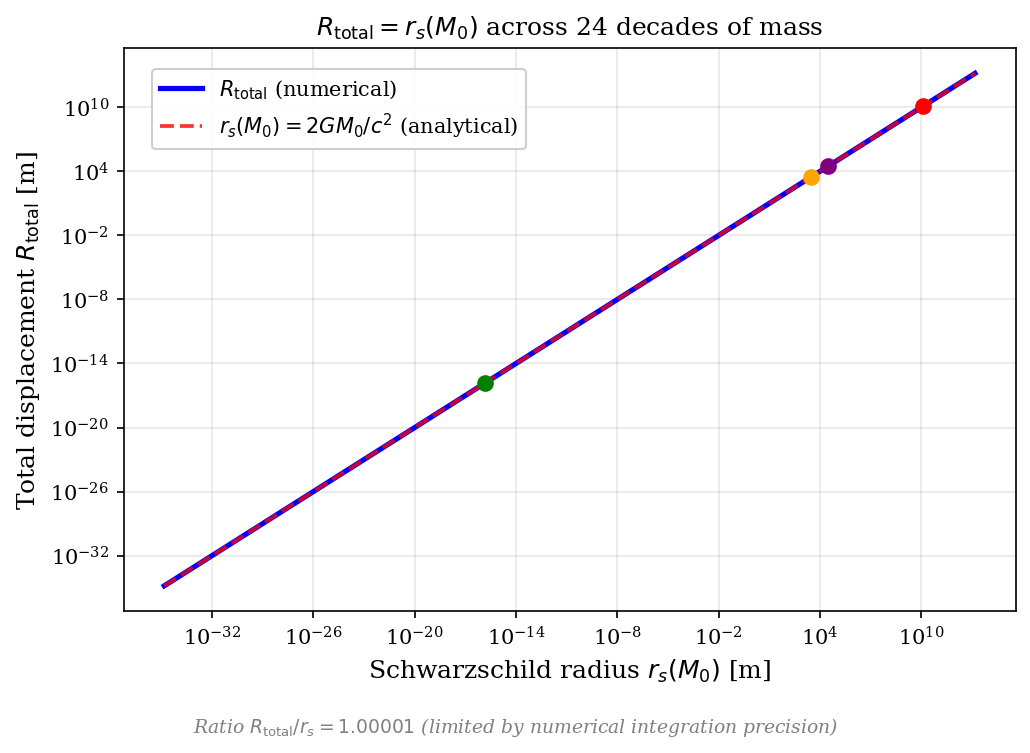
\includegraphics[width=\columnwidth]{fig2_rtotal_vs_rs.png}
\caption{Total D3 displacement $R_{\rm total}$ (computed numerically, solid blue) 
vs analytical Schwarzschild radius $r_s(M_0)$ (dashed red) for 200 black hole 
masses spanning 24 decades. Both lines are indistinguishable, confirming 
$R_{\rm total}/r_s = 1.00001$ (limited by numerical integration precision) 
across the full mass range.}
\label{fig:rtotal}
\end{figure}

%--------------------------------------------------------------------
\section{Dimensional Analysis}
\label{app:dimensional}
%--------------------------------------------------------------------

We verify that the integrand $\mathcal{D}_3\cdot(dN/dM)$ carries dimensions of
length per unit mass, $[\mathrm{m\,kg^{-1}}]$, consistent with $R_{\rm total}$
being a length. Using $[\hbar]=\mathrm{kg\,m^2\,s^{-1}}$, $[c]=\mathrm{m\,s^{-1}}$,
and $[G]=\mathrm{m^3\,kg^{-1}\,s^{-2}}$,
\begin{align}
[\mathcal{D}_3] &= \frac{[\hbar]}{[M][c]}
= \frac{\mathrm{kg\,m^2\,s^{-1}}}{\mathrm{kg}\cdot\mathrm{m\,s^{-1}}}
= \mathrm{m}, \notag\\[4pt]
\left[\frac{dN}{dM}\right] &= \frac{[G][M]}{[\hbar][c]}
= \frac{\mathrm{m^3\,kg^{-1}\,s^{-2}}\cdot\mathrm{kg}}
       {\mathrm{kg\,m^2\,s^{-1}}\cdot\mathrm{m\,s^{-1}}}
= \frac{\mathrm{m^3\,s^{-2}}}{\mathrm{kg\,m^3\,s^{-2}}}
= \mathrm{kg^{-1}}. \notag
\end{align}
Hence $[\mathcal{D}_3\cdot(dN/dM)]=\mathrm{m}\cdot\mathrm{kg^{-1}}=\mathrm{m\,kg^{-1}}$
(the bit count being dimensionless), and
$[R_{\rm total}]=\mathrm{m\,kg^{-1}}\cdot\mathrm{kg}=\mathrm{m}$, a length, as
required. The displacement rate
\begin{equation}
\frac{2G}{c^2}=\frac{2(6.674\times10^{-11})}{(2.998\times10^8)^2}
=1.485\times10^{-27}\ \mathrm{m\,kg^{-1}}
\end{equation}
is the specific Schwarzschild radius --- the horizon radius per unit mass.

%--------------------------------------------------------------------
\begin{thebibliography}{99}

\bibitem{sharma2026d3}
B.~Sharma,
\textit{Geometric Cost of Information Erasure: A Schwarzschild-Radius Formulation 
of the Landauer-Einstein-Schwarzschild Identity},
Zenodo preprint, \href{https://doi.org/10.5281/zenodo.20502577}{DOI:~10.5281/zenodo.20502577} (2026).

\bibitem{bekenstein1973}
J.~D.~Bekenstein,
\textit{Black holes and entropy},
Phys.\ Rev.\ D \textbf{7}, 2333 (1973).

\bibitem{hawking1975}
S.~W.~Hawking,
\textit{Particle creation by black holes},
Commun.\ Math.\ Phys.\ \textbf{43}, 199 (1975).

\bibitem{jacobson1995}
T.~Jacobson,
\textit{Thermodynamics of spacetime: the Einstein equation of state},
Phys.\ Rev.\ Lett.\ \textbf{75}, 1260 (1995).

\bibitem{verlinde2011}
E.~Verlinde,
\textit{On the origin of gravity and the laws of Newton},
JHEP \textbf{04} (2011) 029.

\bibitem{gao2010}
S.~Gao,
\textit{On the falsity of Verlinde's derivation of Newton's law},
arXiv:1002.2668 (2010).

\bibitem{hossenfelder2011}
S.~Hossenfelder,
\textit{Comments on and comments on comments on Verlinde's paper},
Mod.\ Phys.\ Lett.\ A \textbf{26}, 549 (2011).

\bibitem{wheeler1990}
J.~A.~Wheeler,
\textit{Information, physics, quantum: the search for links},
in \textit{Complexity, Entropy, and the Physics of Information},
ed.\ W.~Zurek (Addison-Wesley, 1990).

\bibitem{landauer1961}
R.~Landauer,
\textit{Irreversibility and heat generation in the computing process},
IBM J.\ Res.\ Develop.\ \textbf{5}, 183 (1961).

\bibitem{berut2012}
A.~B\'erut, A.~Arakelyan, A.~Petrosyan, S.~Ciliberto, R.~Dillenschneider, E.~Lutz,
\textit{Experimental verification of Landauer's principle linking information 
and thermodynamics},
Nature \textbf{483}, 187 (2012).

\bibitem{jun2014}
Y.~Jun, M.~Gavrilov, J.~Bechhoefer,
\textit{High-precision test of Landauer's principle in a feedback trap},
Phys.\ Rev.\ Lett.\ \textbf{113}, 190601 (2014).

\bibitem{hong2016}
J.~Hong, B.~Lambson, S.~Dhuey, J.~Bokor,
\textit{Experimental test of Landauer's principle in nanomagnetic memory bits},
Sci.\ Adv.\ \textbf{2}, e1501492 (2016).

\bibitem{neri2016}
I.~Neri, M.~Lopez-Suarez,
\textit{Heat production and error probability relation in Landauer reset at 
effective temperature},
Sci.\ Rep.\ \textbf{6}, 34039 (2016).

\bibitem{cortes2025}
M.~Cort\'es, A.~R.~Liddle,
\textit{Hawking evaporation and the Landauer principle},
EPL \textbf{149}, 59001 (2025); arXiv:2407.08777.

\bibitem{bagchi2024}
B.~Bagchi, A.~Ghosh, S.~Sen,
\textit{Landauer's principle and black hole area quantization},
Gen.\ Relativ.\ Gravit.\ \textbf{56}, 108 (2024); arXiv:2408.02077.

\bibitem{herrera2020}
L.~Herrera,
\textit{Landauer principle and general relativity},
Entropy \textbf{22}, 340 (2020).

\bibitem{kim2010}
H.-C.~Kim, J.-W.~Lee, J.~Lee,
\textit{Black hole as an information eraser},
Mod.\ Phys.\ Lett.\ A \textbf{25}, 1581 (2010); arXiv:0709.3573.

\bibitem{hawking1976}
S.~W.~Hawking,
\textit{Breakdown of predictability in gravitational collapse},
Phys.\ Rev.\ D \textbf{14}, 2460 (1976).

\bibitem{page1993}
D.~N.~Page,
\textit{Information in black hole radiation},
Phys.\ Rev.\ Lett.\ \textbf{71}, 3743 (1993).

\bibitem{penington2020}
G.~Penington,
\textit{Entanglement wedge reconstruction and the information paradox},
JHEP \textbf{09} (2020) 002.

\bibitem{almheiri2019}
A.~Almheiri, N.~Engelhardt, D.~Marolf, H.~Maxfield,
\textit{Entanglement wedge as the bulk dual of the boundary density matrix},
JHEP \textbf{01} (2019) 149.

\bibitem{klaers2019}
J.~Klaers,
\textit{Landauer's erasure principle in a squeezed thermal memory},
Phys.\ Rev.\ Lett.\ \textbf{122}, 040602 (2019).

\end{thebibliography}

\end{document}
